%  Document History:
%
%-----------------------------------------------------------------------
\documentclass[a4paper,twoside]{arlims}
%------------------------------------------------------------------------- 

%--- Settings for the ARLIMS document class ---
\setcounter{page}{101} % The starting page

%--- This part of the preamble can be fiddled with according to our needs ---

% Some packages that we like and wan to use:
\usepackage{cite}
\usepackage{url}
\usepackage{graphicx}

% The path(s) to the graphics files:
\graphicspath{{eps/}{pdf/}}

% correct bad hyphenation here
\hyphenation{op-tical net-works semi-conduc-tor}

% This makes line breaks look prettier
\sloppy

%--- Preamble definitions for actual content ---

\title{Your Title}

\author{Your I. Name}
\authorB{, An Othername}
\authorC{ and Third Author}

\institute{Computer Science\\
Institute of Information \& Mathematical Sciences\\
Massey University at Albany, Auckland, New Zealand\\
Email: \textnormal{\texttt{\{Y.I.Name | A.Othername | T.Author\}@massey.ac.nz}}}

%------------------------------------------------------------------------- 
\begin{document}

% Put a proper title on the first page:
\maketitle

%------------------------------------------------------------------------- 
\begin{abstract}
  Your abstract here. Your abstract here. Your abstract here. Your
  abstract here. Your abstract here. Your abstract here. Your abstract
  here. Your abstract here. Your abstract here.
  
  \paragraph{Keywords:} small-worlds; computational Grid services; online
  communities; sparse matrices.
\end{abstract}

%------------------------------------------------------------------------- 
\section{Introduction}
\label{sect:Introduction}

OK, start out writing your document here. And to show off a little I
will reference this \cite{sparse-survey} for our immediate pleasure.

Blah. Blah. Blah. Blah. Blah. Blah. Blah. Blah. Blah. Blah. Blah.
Blah. Blah. Blah. Blah. Blah. Blah. Blah. Blah. Blah. Blah. Blah.
Blah. Blah. Blah. Blah. Blah. Blah. Blah. Blah. Blah.

Blank lines indicate paragraphs.

Blah. Blah. Blah. Blah. Blah. Blah. Blah. Blah. Blah. Blah. Blah.
Blah. Blah. Blah. Blah. Blah. Blah. Blah. Blah. Blah. Blah. Blah.
Blah. Blah. Blah. Blah. Blah. Blah. Blah. Blah. Blah. Blah. Blah.
Blah. Blah. Blah. Blah. Blah. Blah. Blah. Blah. Blah. Blah. Blah.
Blah. Blah. Blah. Blah. Blah. Blah. Blah. Blah. Blah. Blah. Blah.
Blah. Blah. Blah. Blah. Blah. Blah. Blah. Blah. Blah.


\section{System Architecture}
\label{sect:Architecture}

Here we've got some sub sections in the document as well.


\subsection{A Figure}
\label{subsect:Figure}

And this is Fig. \ref{fig:timing}, as you can see ...

\begin{figure}[hbt]
  \centering
  % It is going to be 75% of the text's width and called "timing" ...
  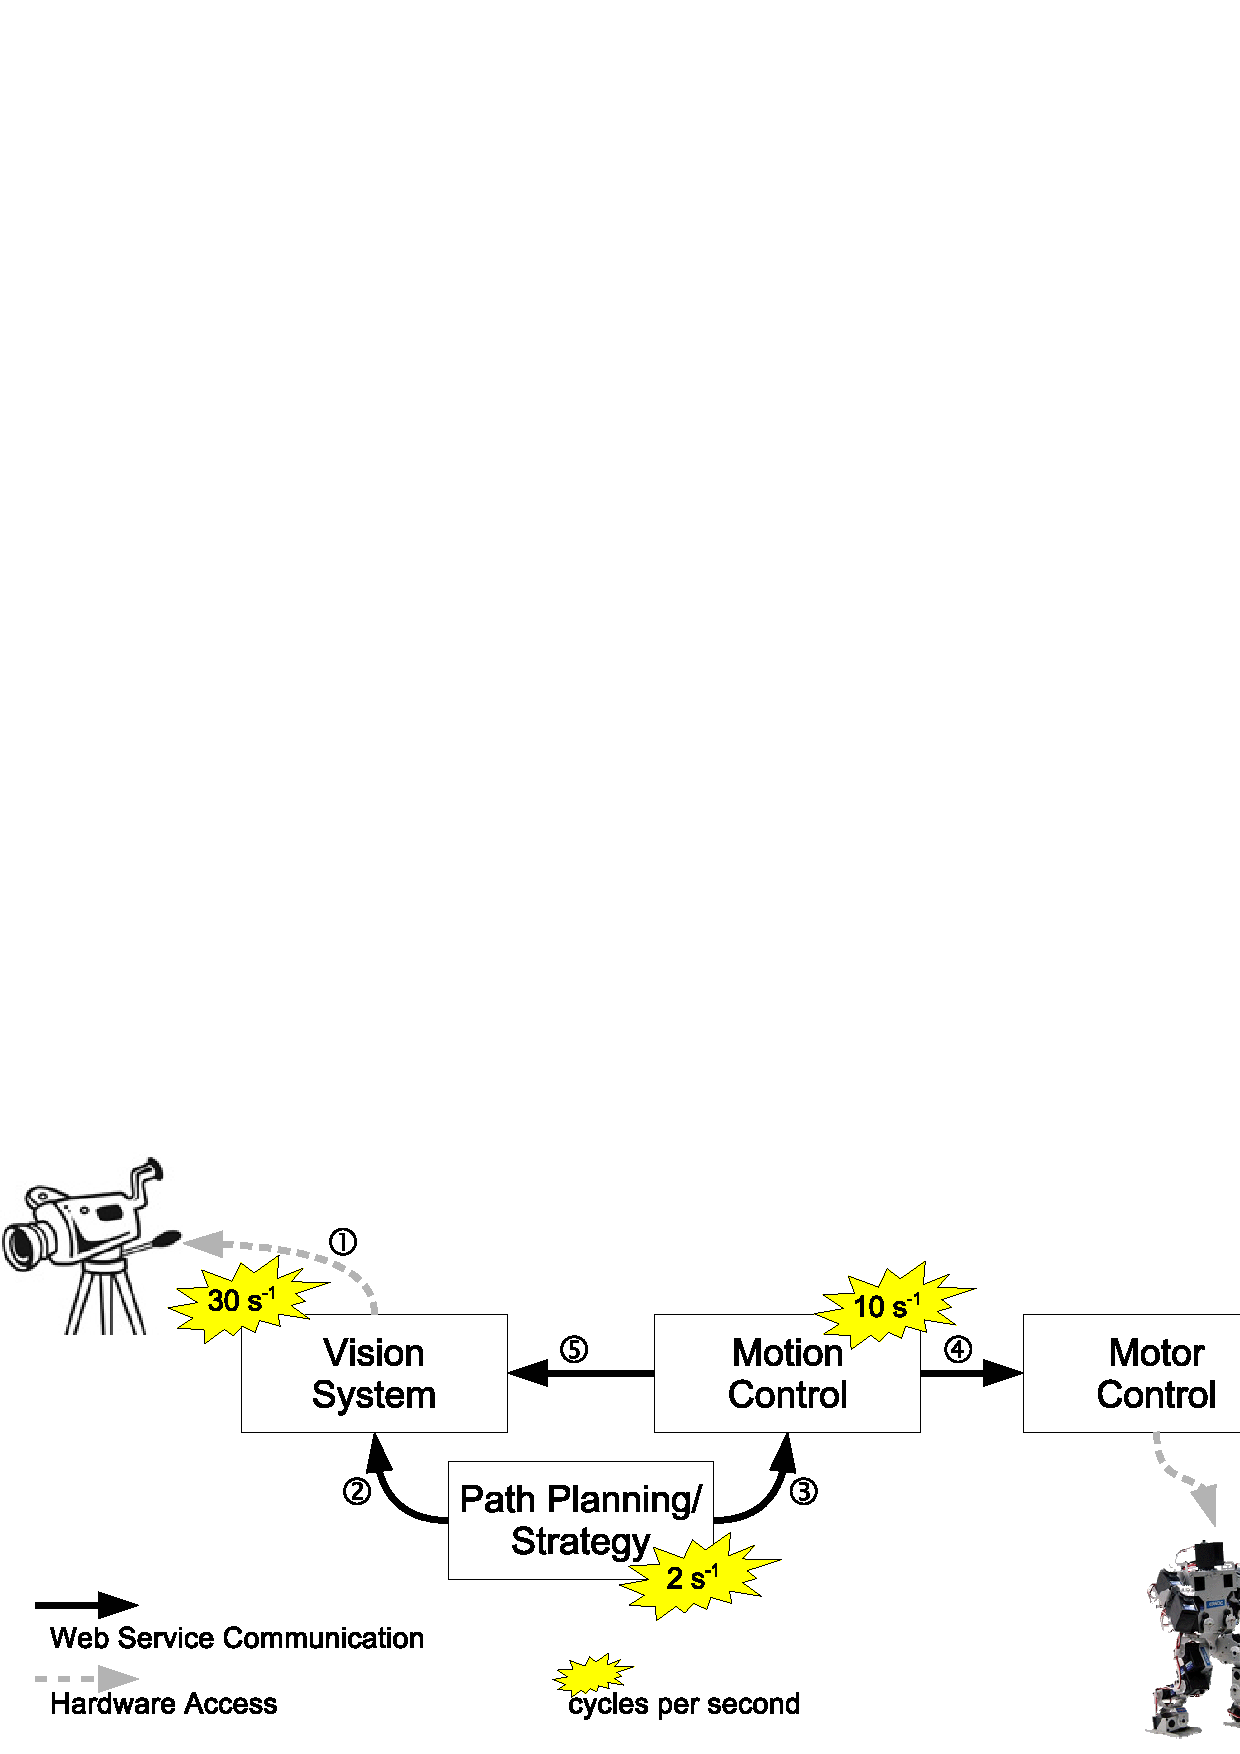
\includegraphics[width=.75\hsize]{timing}
  \caption{Distribution of workflow components on the network.}
  % Look above, this is how we can reference it by a label ...
  \label{fig:timing}
\end{figure}


\subsection{A Table}
\label{subsect:Table}

And this is Table \ref{tab:LINALG}, as you can see ...

\begin{table*}[htbp]
  \caption{Linear Algebra Grid Services}
  \centering
  \begin{tabular}{|l|c|l|}
    \hline
    \textbf{Example Linear Algebra Services} & \textbf{Data Types} & \textbf{Resource Requirement} \\
    \hline
    Store a Matrix as part of a calculation  & M          &   Temp storage            \\
    Store a Vector as part of a calculation  & V          &   Temp storage            \\
    Store or retrieve a particular matrix    & M          &   Long term storage       \\
    Extract particular value from a matrix   & M :        &   Compute                 \\
    Dense Matrix-Vector Multiply             & M, V: V    &   Compute + Temp Storage  \\
    Dense Matrix-Matrix Multiply             & M, M: M    &   Compute + Temp Storage  \\
    Dense Matrix Invert                      & M : M      &   Compute + Temp Storage  \\
    Dense Matrix Solve                       & M, V: V    &   Compute + Temp Storage  \\
    Sparse Matrix to Dense Matrix Expand     & S: M       &   Compute + Temp Storage  \\
    Sparse Matrix Conjugate Gradient Solve   & S, V: V    &   Compute + Temp Storage  \\
    \hline
  \end{tabular}
  % Tables also like to have a label to be referenced ...
  \label{tab:LINALG}
\end{table*}


\section{Conclusions and Summary}
\label{sec:conclusions}

Of course you want to conclude, don't you? 

Blah. Blah. Blah. Blah. Blah. Blah. Blah. Blah. Blah. Blah. Blah.
Blah. Blah. Blah. Blah. Blah. Blah. Blah. Blah. Blah. Blah. Blah.
Blah. Blah. Blah. Blah. Blah. Blah. Blah. Blah. Blah. Blah. Blah.
Blah. Blah. Blah. Blah. Blah. Blah. Blah. Blah. Blah. Blah. Blah.
Blah. Blah. Blah. Blah. Blah. Blah. Blah. Blah. Blah. Blah. Blah.
Blah. Blah. Blah. Blah. Blah. Blah. Blah. Blah. Blah.


%------------------------------------------------------------------------- 
\section*{Acknowledgements}
None in particular. But this section has got an asterisk in the
code, and this way it does not get numbered by \LaTeX.


%------------------------------------------------------------------------- 
%--- back matter: bibliography ---
% These are in alphabetical by leading author order.
\bibliographystyle{plain}
\begin{thebibliography}{10}

\bibitem{sparse-survey} 
  Barrett, R., Berry, M., Chan, T.F., Demmel, J., Donato, J.,
  Dongarra, J., Eijkhout, V., Pozo, R., Romine, C., van der Vorst, H.
  ``Templates for the Solution of Linear Systems: Building Blocks for
  Iterative Methods,'' SIAM, Philadelphia, PA, 1994.


\end{thebibliography}

%------------------------------------------------------------------------- 
% We need this for the style to work properly, so please leave it in here:
\label{lastpagenum}
\end{document}
